% Progress Report
% CS 461 - CS Senior Capstone
% Fall 2017
% Authors: Connor Christensen, Lily Shellhammer, William Buffum


\documentclass[draftclsnofoot,onecolumn,letterpaper,10pt,compsoc]{IEEEtran}

% Packaging
\usepackage{geometry}
\usepackage{hyperref}
\usepackage{titling}
\usepackage{color}
\usepackage{listings}
\usepackage{cite}
\usepackage{pdfpages}
\usepackage{pdflscape}
\usepackage{url}
\usepackage{array}
\usepackage{graphicx}
\usepackage{subfig}

\definecolor{lightgray}{rgb}{0.95,0.95,0.95}
\definecolor{darkgray}{rgb}{0.5,0.5,0.5}
\definecolor{softred}{rgb}{0.7,0,0}

\lstdefinelanguage{JavaScript}{
  keywords={typeof, new, true, false, catch, function, return, null, catch, switch, var, if, in, while, do, else, case, break},
  keywordstyle=\color{blue}\bfseries,
  ndkeywords={class, export, boolean, throw, implements, import, this},
  ndkeywordstyle=\color{darkgray}\bfseries,
  identifierstyle=\color{black},
  sensitive=false,
  comment=[l]{//},
  morecomment=[s]{/*}{*/},
  commentstyle=\color{purple}\ttfamily,
  stringstyle=\color{red}\ttfamily,
  morestring=[b]',
  morestring=[b]"
}

\lstset{
   language=JavaScript,
   backgroundcolor=\color{lightgray},
   extendedchars=true,
   basicstyle=\footnotesize\ttfamily,
   showstringspaces=false,
   showspaces=false,
   numbers=left,
   numberstyle=\footnotesize,
   numbersep=9pt,
   tabsize=2,
   breaklines=true,
   showtabs=false,
   captionpos=b
}

\lstdefinelanguage{Stylus}{
  keywords={@media},
  keywordstyle=\color{blue}\bfseries,
  ndkeywords={px},
  ndkeywordstyle=\color{softred}\bfseries,
  identifierstyle=\color{black},
  sensitive=false,
  comment=[l]{//},
  morecomment=[s]{/*}{*/},
  commentstyle=\color{purple}\ttfamily,
  stringstyle=\color{red}\ttfamily,
  morestring=[b]',
  morestring=[b]"
}

\lstset{
   language=Stylus,
   backgroundcolor=\color{lightgray},
   extendedchars=true,
   basicstyle=\footnotesize\ttfamily,
   showstringspaces=false,
   showspaces=false,
   numbers=left,
   numberstyle=\footnotesize,
   numbersep=9pt,
   tabsize=2,
   breaklines=true,
   showtabs=false,
   captionpos=b
}

% Paper type
\geometry{letterpaper, margin=.75in}

% Title page
\title{CS 461 - CS Senior Capstone
	\\Fall 2017
	\\Progress Report
}


\author{
	Connor I. Christensen \\
	\texttt{chriconn@oregonstate.edu}
	\\
	Lily M. Shellhammer \\
	\texttt{shellhal@oregonstate.edu}
	\\
	William B. Buffum \\
	\texttt{buffumw@oregonstate.edu}
}

\begin{document}
\begin{titlingpage}
    \maketitle
    \begin{abstract}
			Ninkasi Brewing Company is based in Eugene, Oregon, producing and distributing nearly 100,000 barrels of beer each year across the United States and Canada.
			Ninkasi currently tracks brewery data using digital spreadsheets, a laborious, time consuming, and error prone process.
			Quality brewing requires the company to be detail-oriented, organize its data and provide timely actions in the brewing process.
			In order to maintain good quality control in their product and give the company room to scale in its production, our team has been tasked with creating software that will improve the process of entering, storing and accessing data related to the brewing process.
			This document examines work completed on the project to this date.
			At this point in the middle of the winter term, our product has reached an alpha state and has a working interface with no database connections.
			Throughout this Progress Report, readers will see a week-by-week recount of the preparation completed for Winter term.
			\\
			\textbf{Keywords:} Brewing, Operations Management, Web App
    \end{abstract}
		\pagebreak
		\tableofcontents
\end{titlingpage}

% briefly recaps the project purposes and goals
% describes where you are currently on the project
% describes what you have left to do
% describes any problems that have impeded your progress, with any solutions you have
% includes particularly interesting pieces of code (if coding is involved)
% (research only) includes descriptions of experimental design
% (interface design only) includes description of first user study, hopefully with results
% includes images of your project -- screen shots, photos, whatever is appropriate

\section{Introduction}
\subsection{Purpose}
\subsection{Scope}
\subsection{Overview}
Provide a recap of the project purposes and goals. \\

\section{Connor Christensen}
\subsection{Current position in the project timeline}

Our app is split into three different components, with each member of the team working on their own component. There is the front end, back end, and the JavaScript framework between them.
Out of those three components, the front end is the most complete, with the app comfortably in alpha.
The user interface will not be fully functional until data can be retrieved from the database and injected into the site, but the app looks very similar to the designs.
The app is currently utilizing a small amount of Vue.js to detect whether it is running on a mobile device and adapts the content accordingly.
If Vue detects that it is running on a mobile device, it takes distinct components from single pages and splits them into separate pages, so everything can be accessed on the mobile device without the need to scroll.


The elements I have worked on since the beginning of the term has been the design process that I worked on for a month over winter break, and the last five weeks I have spent implementing that design.
I set up the file structure, task runner, wrote the html and css to style the interface, and integrated Vue components and routing into the project.
The next few paragraphs explain in more detail each of the elements I have worked on and what they do in the scope of the project.


Vue components are fully encapsulated html and css templates with an associated instance of a Vue object.
These components can be integrated together into other components or into web pages.
For example, the homepage for the desktop contains both the data entry and tank monitoring components.
Defining these as components keeps the webpages modular, with very low chances of elements on the page interacting with other elements in unintended manners.
Another benefit to Vue components is that each component can be registered as a component to a page, or its own page.
This means that a web page can easily be split up into smaller pages that are easier to access on mobile.
I have been testing the site both on mobile and desktop versions as I go to ensure that I don't focus too much on a particular representation of the site.


Routing is behavior that uses JavaScript to mimic a multi-page website without ever requiring the app to refresh the page or make a request to a server.
There is never any redirecting to a different URL, which is how the mobile and desktop utilize the same codebase while having tailored experiences on both devices.
Each component is registered for its own route, while also serving as components in the desktop version of the pages.


Webpack is integrated in the project to compile the Vue files down into their respective html, css and JavaScript files.
Webpack provides a method to live render our site on our own machines through a port on localhost during development, while also giving the option of creating highly minified files ready for deployment.


Given the highly modular nature of this project, and the simple requirements for buttons, input fields and some data display, all the styling was written manually.
This gave the most amount of control to be able to fit exactly what had been decided in the design stage with the client.
The css is written in stylus, which is a css preprocessor that has some functionality as well as aesthetic benefits for the language itself.




\subsection{What is left to do}


The user interface is in its final stages, so the team will focus most of its energy on finishing the tasks needed to be able to reach a minimum viable product.
Once the minimum viable product is reached, then the team can focus on stretch goals.
A majority of the work needs to be done on the back and middle end sections, but there are a few improvements left to make to the interface such as making sure the app always runs on full screen mode on mobile devices.
After I finish up the few features I have left to work on, I will be sending the prototype over to Ninkasi sometime in the next few weeks, so they can give me feedback.
Though we have spent several iterations agreeing on a design, it is frequent that a client might have a few more suggestions when they experience the product in a more interactive form.


\subsection{Problems encountered and solutions to those problems}

Currently, there are no issues for me that impede my work.
In order for the interface to be done, Lily needs to make some modifications and additions to the Vue code in order to make the site more reactive.


The biggest problem I have run into so far was integrating routing into the project.
When the project was first created, I started utilizing Gulp as our task runner.
It would be in charge of compiling, compressing and making it easy to develop and deploy our code.
This worked great when I was writing the user interface in html and stylus, but when I went to add in Vue components and get routing working on the site, I had a lot of difficulty.
It was sometimes working, and when it was not working, it was breaking in very strange ways.
I decided that it was not in our best interest as a team to be using a task-runner that was being incrementally developed by me in unusual ways to make it work.
I took a lot of time to think about how to approach this problem from a few steps back and found that Vue already had a command line interface tool that would allow for easy development of Vue components with the help of webpack.
Changing over to webpack was not an easy decision, as it involved completely restructuring what I had done so far.
The html and stylus code were still usable, but it needed some serious rearranging in order to make it work in the new structure.



\subsection{Particularly interesting pieces of code}

This is the strange single if statement that checks to see whether the device running the site is any form of mobile device.
Inside this if statement is the processes of setting routes on links in the page and switching a boolean to true that determines what little components are shown or hidden.

\lstset{language=JavaScript}
\lstinputlisting{mobile.js}

Some code that is particularly impressive in this project is some custom code that was written to improve the ease of use with which to use media queries in css.
Media queries are used to define specific rules that should be taking place only under certain circumstances.
They are most commonly used as if statements with regards to screen size.


After tinkering with breakpoints, using the traditional media screen definition is consistently confusing and the sizes at which the breakpoints are enacted tend to happen at fairly random screen sizes.
The breakpoints stylus file has some breakpoint variables defined at common screen sizes, and there are three mixins defined that make css breakpoint rules easily readable.

\lstset{language=Stylus}
\lstinputlisting{breakpoints.styl}

Finally, there is some stylus code for defining the number of boxes visible in the tank monitoring page at a variety of page sizes.
If nothing else, I like this code just for how pretty it is.
Using the mixins and variables defined above, it is easy to see exactly which lines are being used by these breakpoints, at what size the breakpoints begin working, and in which direction the rules apply.

\centerline{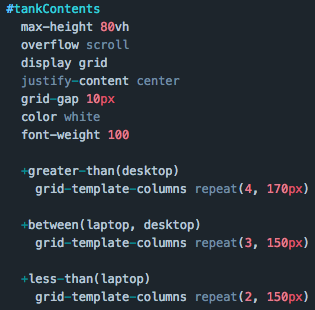
\includegraphics[height=5cm]{screenshots/stylus.png}}

\section{Lily} 
\subsection{Describe where you are currently on the project}
At the start of this term we had our technologies picked out, but hadn’t started on any coding. Connor had mock-ups of the UI design and was ready to launch into that. At this point in the term, our app looks almost identical to our proposed final product, but lacks the data entry functionality. Clicking on navigation buttons leads you to different pages that display the login, tank statuses, data entry form, and data visualizations. The tank status page and visualizations are filled with dummy values. Now that Connor’s work on the front end design is finished, we are working toward finishing building our database, connecting it to our web app via REST API, and validating user input. Billy has completed setting up our server and building the login information part of the database, and the next step is to pull information about users to the login page to validate login credentials. My role in this project is to develop the middle stack, using Vue.js to connect Connor’s website skeleton with Billy’s database. I have worked on creating the main Vue object for our javascript and binding user input to variables. I use javascript to check input fields on the client’s side before (once this functionality is developed) packaging up those variables in a json object and submitting them into the database. My progress so far is learning about Vue and building Vue components, as well as creating the data variables and functions that validate user input.

\subsection{Describe what you have left to do}
My next steps include connecting the database with the front end. I need to begin pulling login information from the database using a REST API. The REST API queries the database and generates a json object. I will validate the user’s login information against the values in those json objects from our database. Then I will use the same system to display tank information and allow the user to submit data about each tank, updating the tank information page and displaying any alerts that need to appear. In order to complete these tasks, I need to learn more about how vue components interact with one another. I also need to learn how to build a json object using vue variables. In order to test how the page runs with many tanks (as we currently have dummy data for only 6) I will write a script that creates 100 json objects filled with random data. Then we can check how the app handles displaying lots of information that it has to pull from the database in that moment.  


\subsection{Describe any problems that have impeded your progress, with any solutions}
For the first two weeks of the term I had a really difficult time getting my environment set up with the frameworks needed to run our web app locally. I eventually had to factory reset my computer because there were so many issues. That process, and the process of setting up the environment from scratch took a lot of time and delayed my coding. 

Connor developed routing through Vue that, based on screen size, displays different vue object components. On mobile, only tank status or the form page are displayed. On a desktop, both the tank status and form page are displayed side by side. Desktop computers also display charts, generated using C3, displaying data over time. The problem Connor has encountered is that using this method of routing does not allow for an easy way of changing the header. Either all pages have the same header, or the child vue component has to pass information to the parent (called emissions) vue component about what page it is on and what size screen, that way the correct header is displayed. Connor and I are brainstorming ways of fixing this problem. Our current idea is to have the header have all types of header information that get triggered by an if statement based on child emissions about page content and screen size. It isn’t very elegant, but it would fix the problem of incorrect headers. 

\subsection{Include particularly interesting pieces of code}
Vue is an easy-to-use object oriented javascript language. You create one Vue object for the whole app and components of the vue app contain different pages information. For example, if you have a form, you can save the templated html with the javascript functionality in a component and display that component whenever the user navigates to the form page. In our case, this is useful because we want to display multiple components on desktops, but only one component on smaller mobile devices. 
My main job so far has been creating a Vue object and client-side form validation functionality. Here is an example of a function validating temperature input:


\centerline{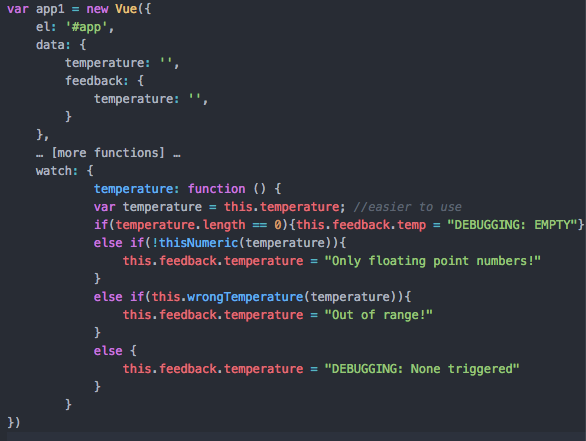
\includegraphics[height=5cm]{screenshots/vuecode.png}}

The Vue object has two-way-binding which means whenever a data variable is changed (either in the object or by the user) it is updated in both places. This makes client-side form verification easy because we can call the “watch” function whenever a variable is changed by the user. This means instant error checking before we send any variables to the database. We can check for bad integers, values out of the acceptable range, and empty input fields. Because we can accept values as strings and then later convert them to numbers, users can type in values for every field and not rely on clunky numeric input mechanisms.

\section{William Buffum}
\subsection{Current position in the project timeline}
\subsection{What is left to do}
\subsection{Problems encountered and solutions to those problems}
\subsection{Particularly interesting pieces of code}

\section{Conclusion}

\subsection{Images of the product}
\centerline{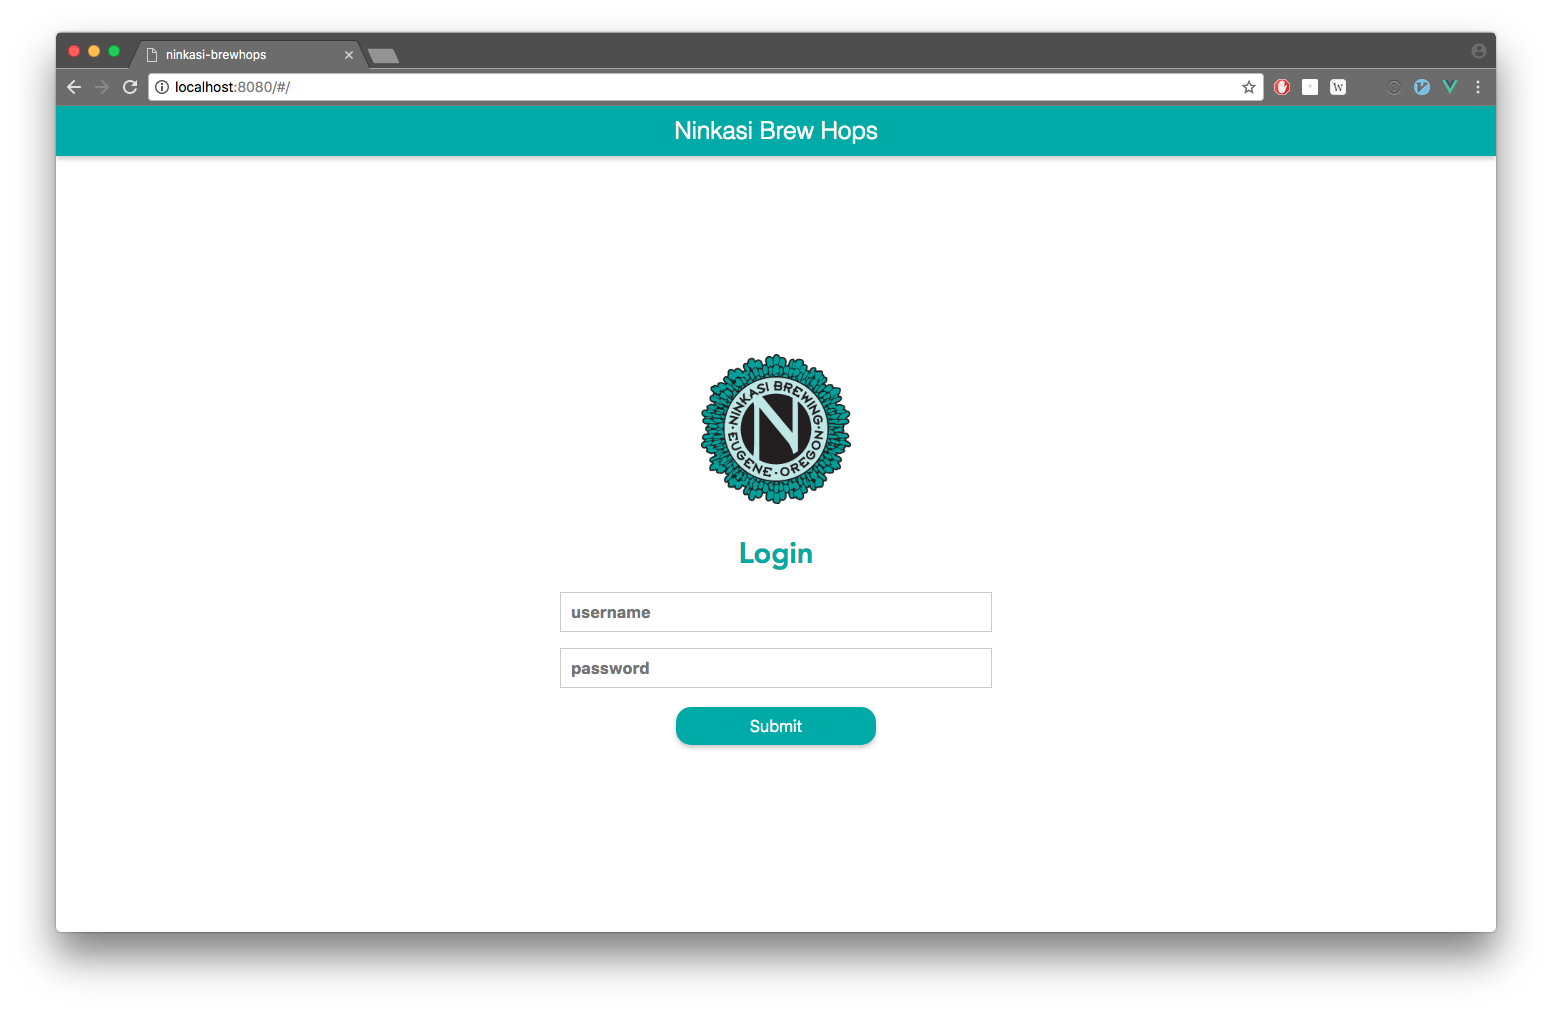
\includegraphics[height=10cm]{screenshots/desktop/login.png}}
\centerline{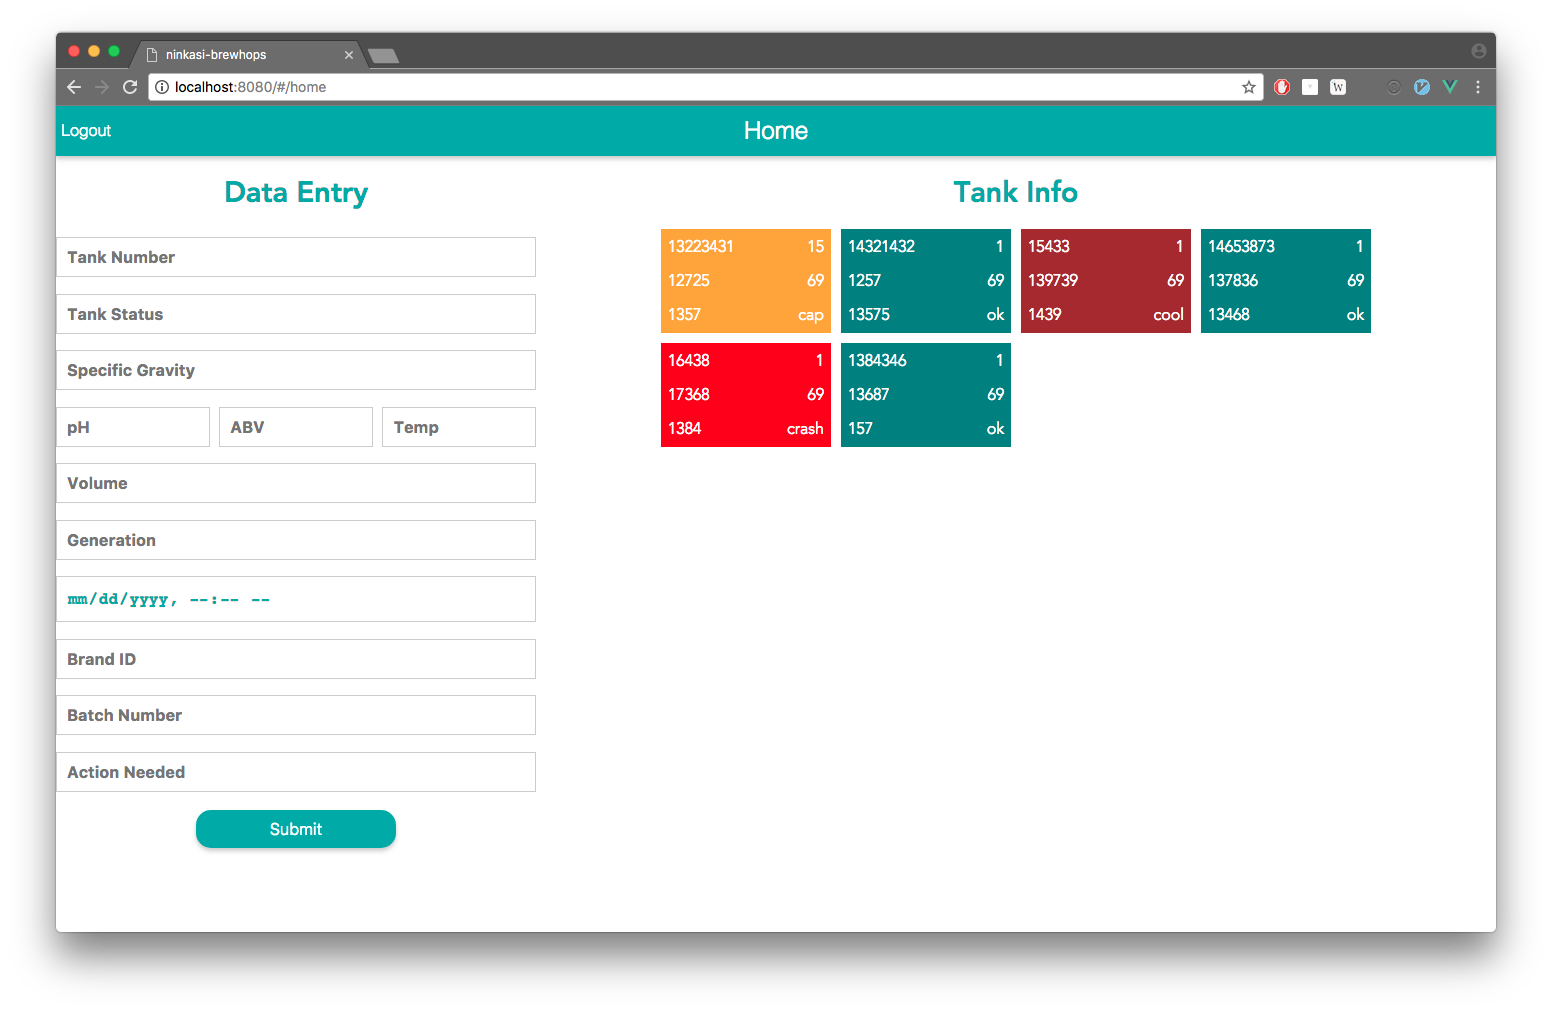
\includegraphics[height=10cm]{screenshots/desktop/home.png}}
\centerline{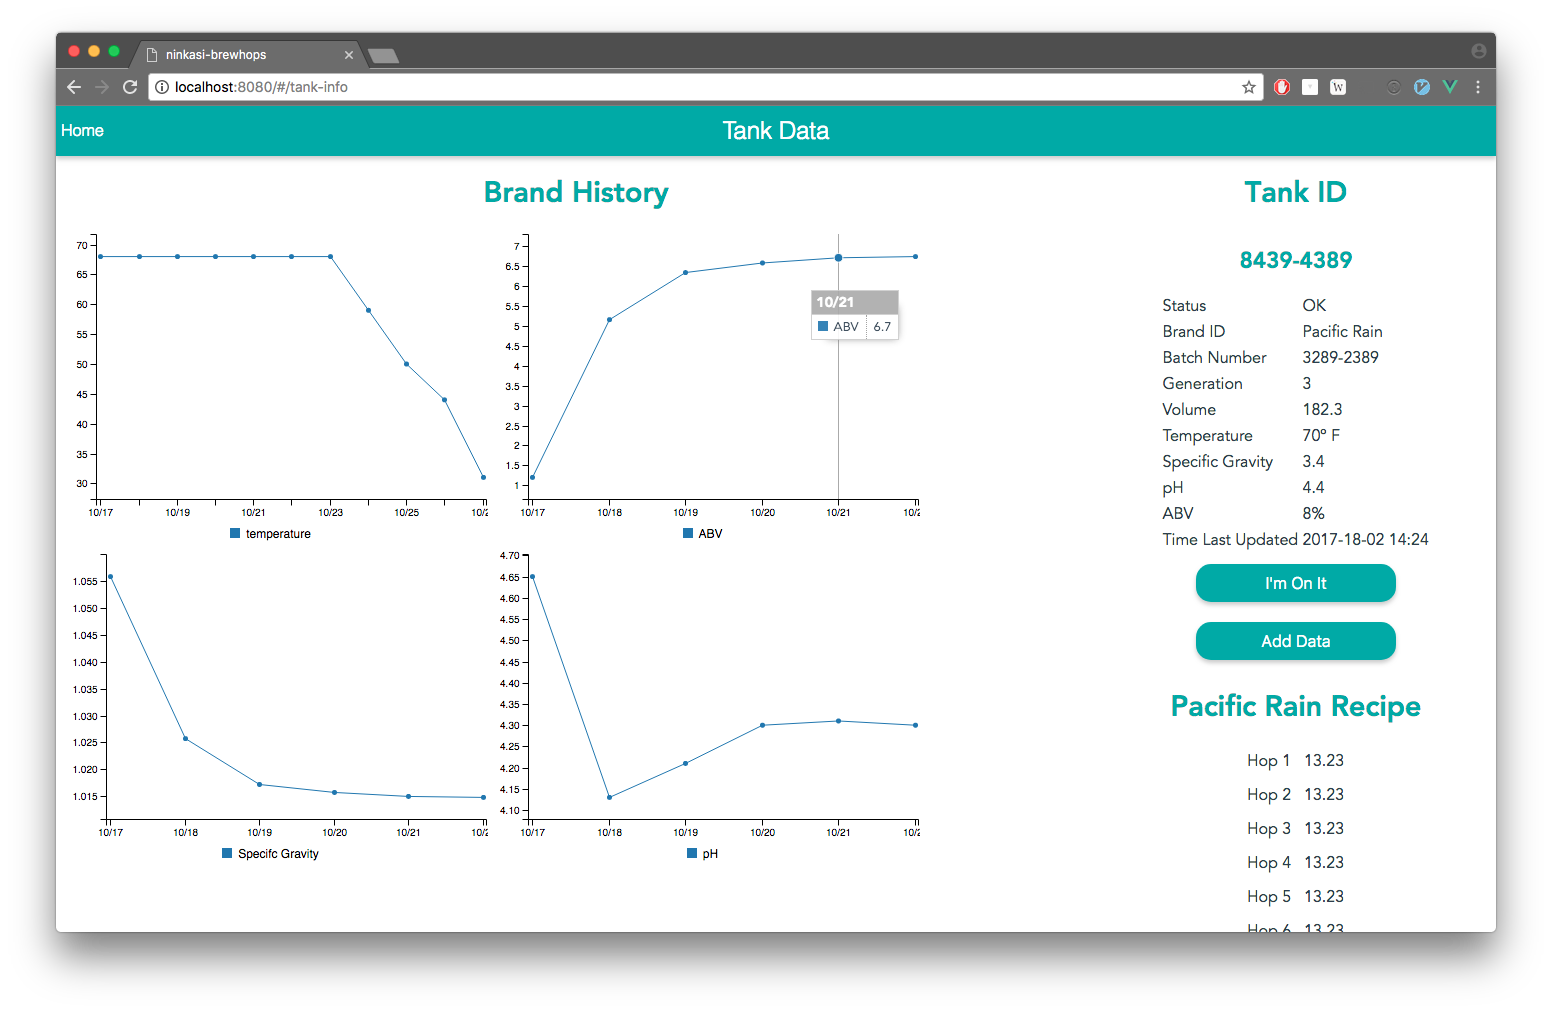
\includegraphics[height=10cm]{screenshots/desktop/tank_info.png}}
\centerline{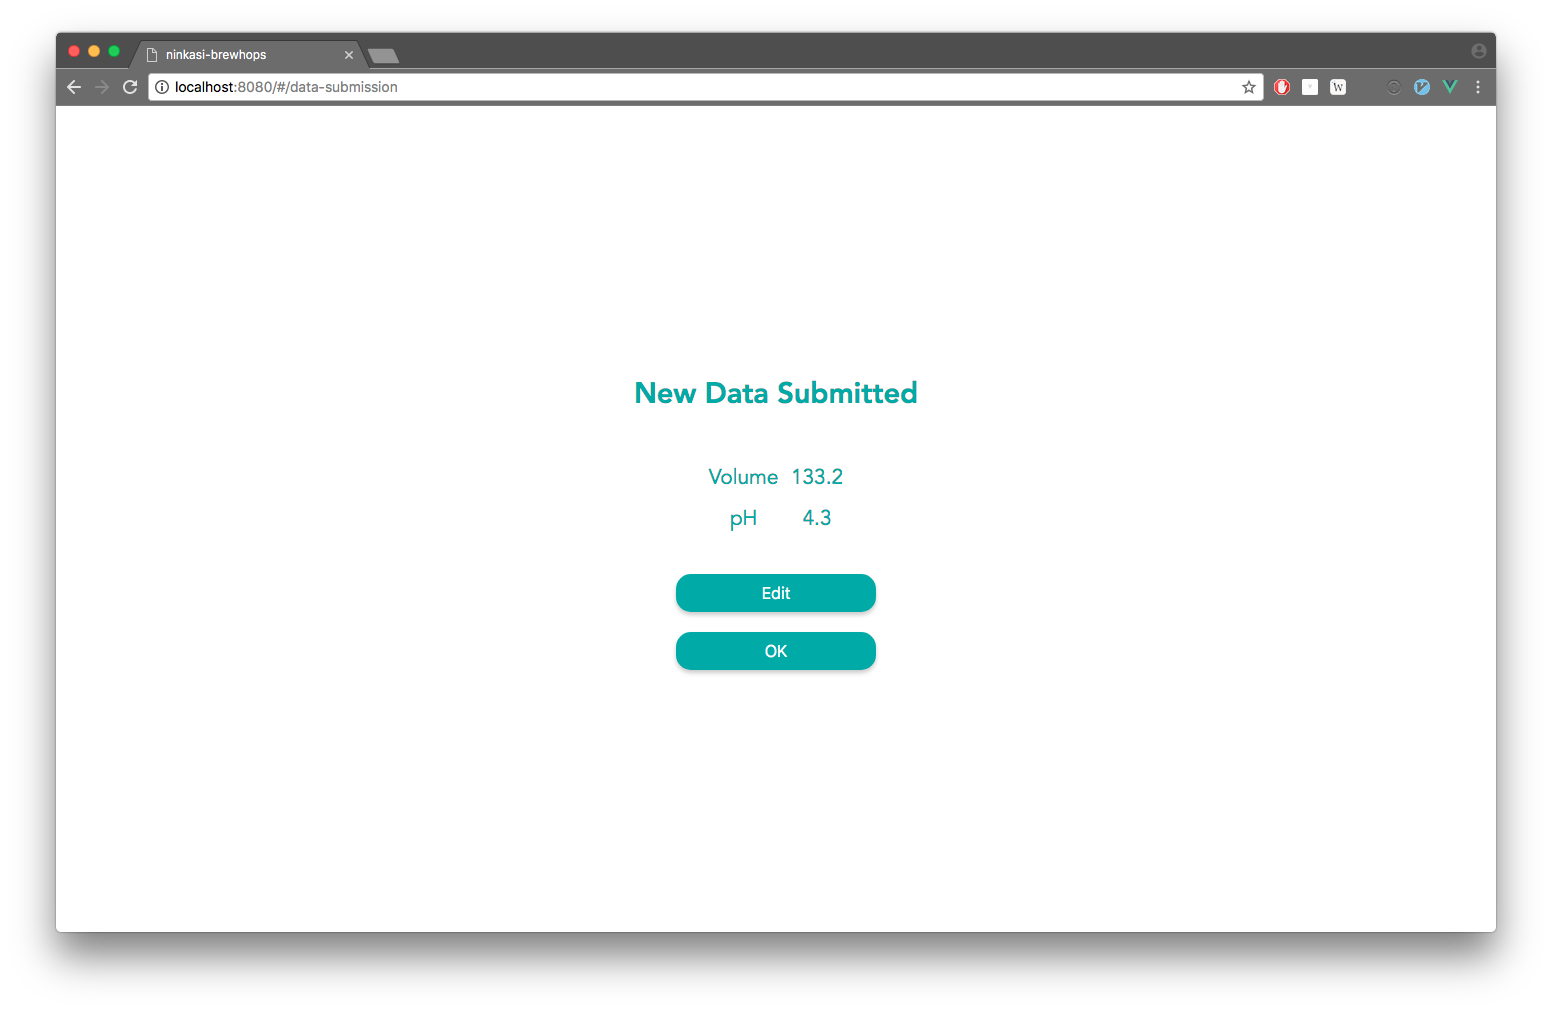
\includegraphics[height=10cm]{screenshots/desktop/data_submission.png}}


\begin{figure}%
    \centering
    \subfloat[Login]{{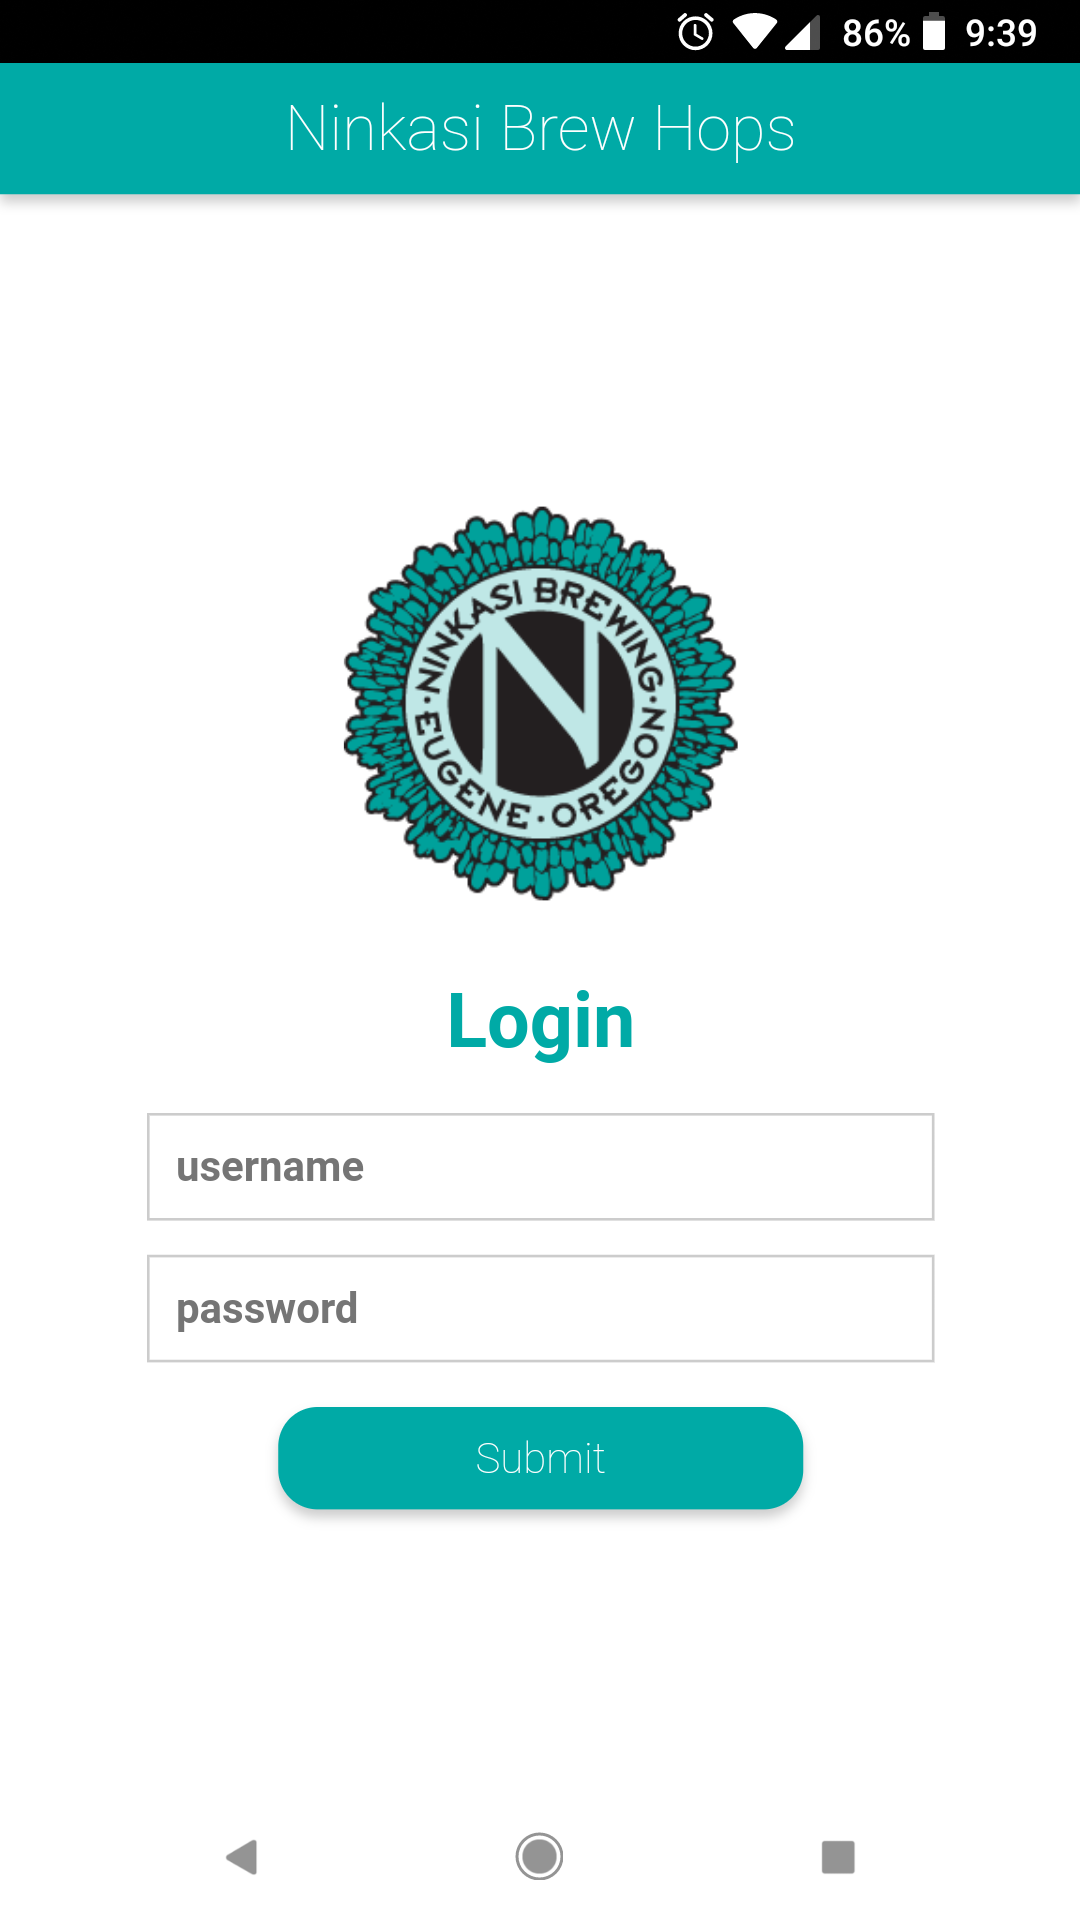
\includegraphics[height=13cm]{screenshots/mobile/login.png}}}%
    \qquad
    \subfloat[Home]{{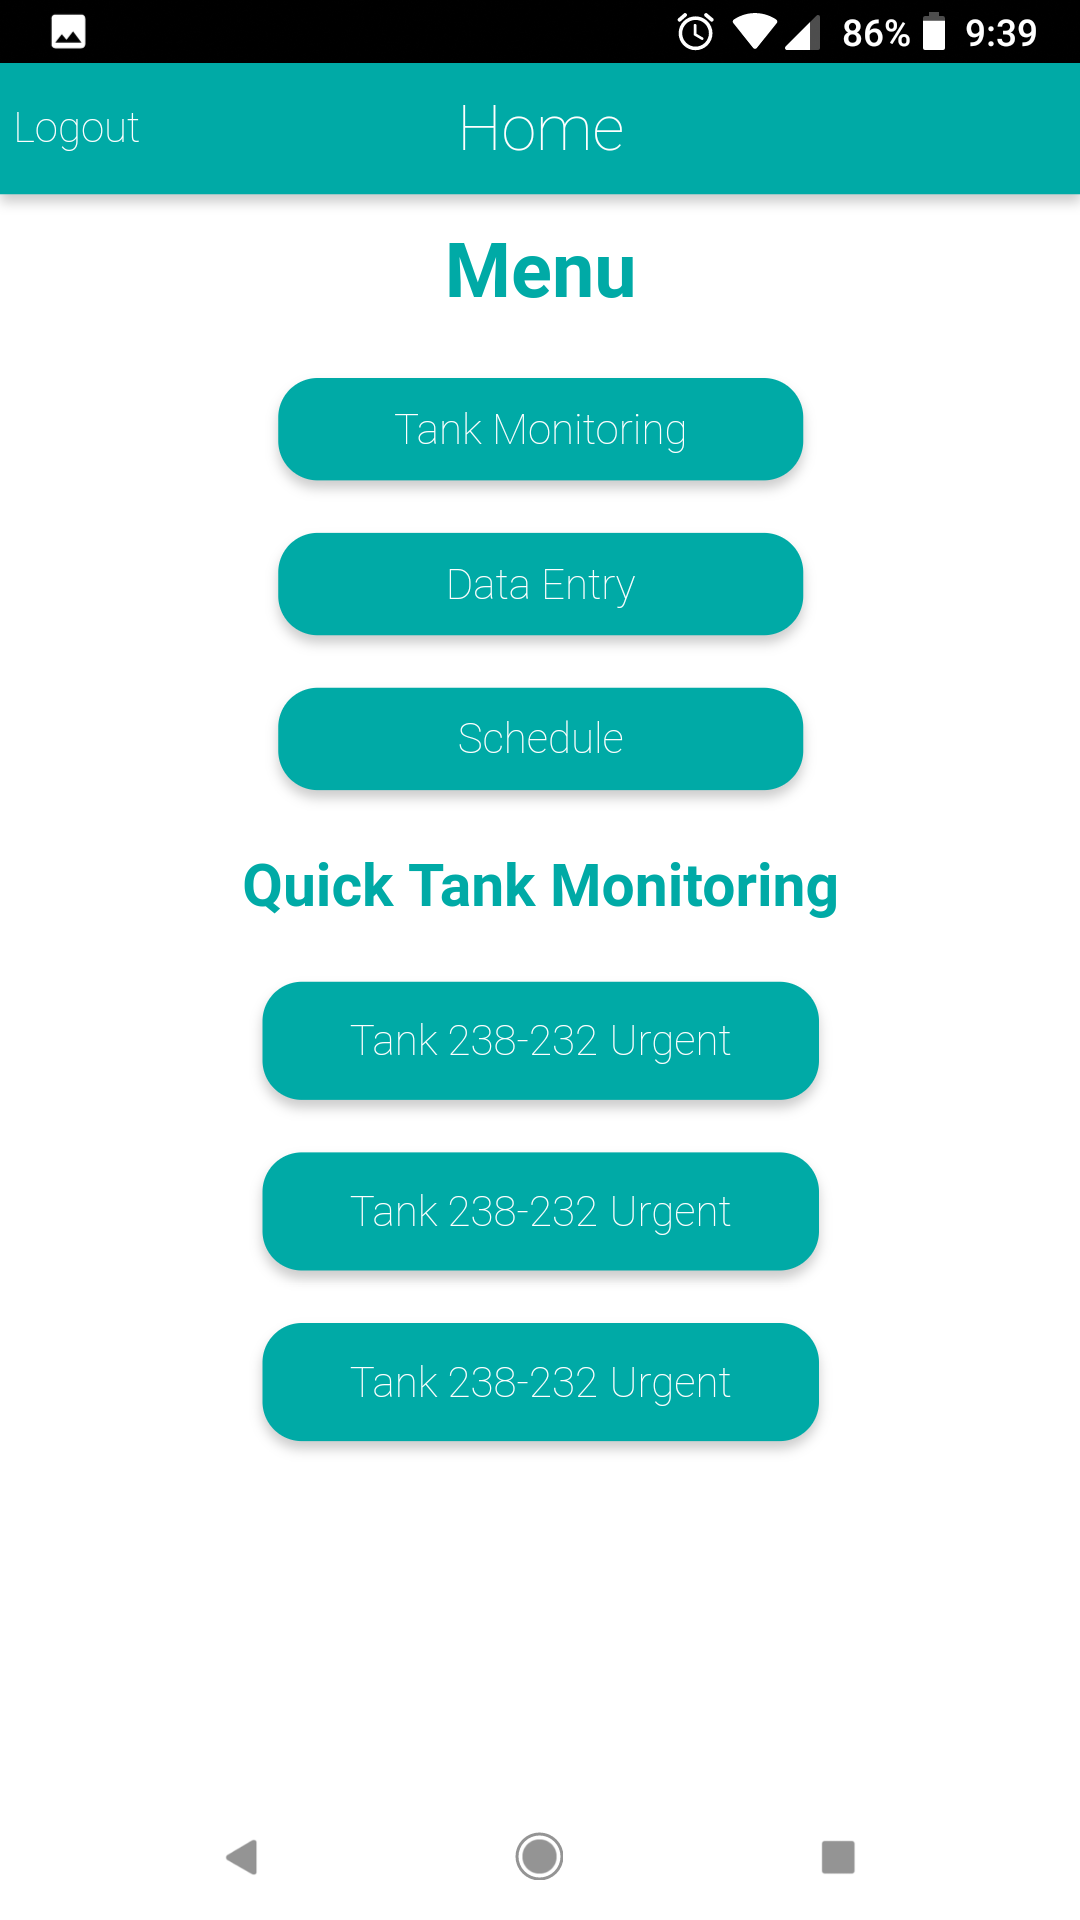
\includegraphics[height=13cm]{screenshots/mobile/home.png}}}%
    \caption{Mobile - Login and Home page}%
\end{figure}

\begin{figure}%
    \centering
    \subfloat[Tank Monitoring]{{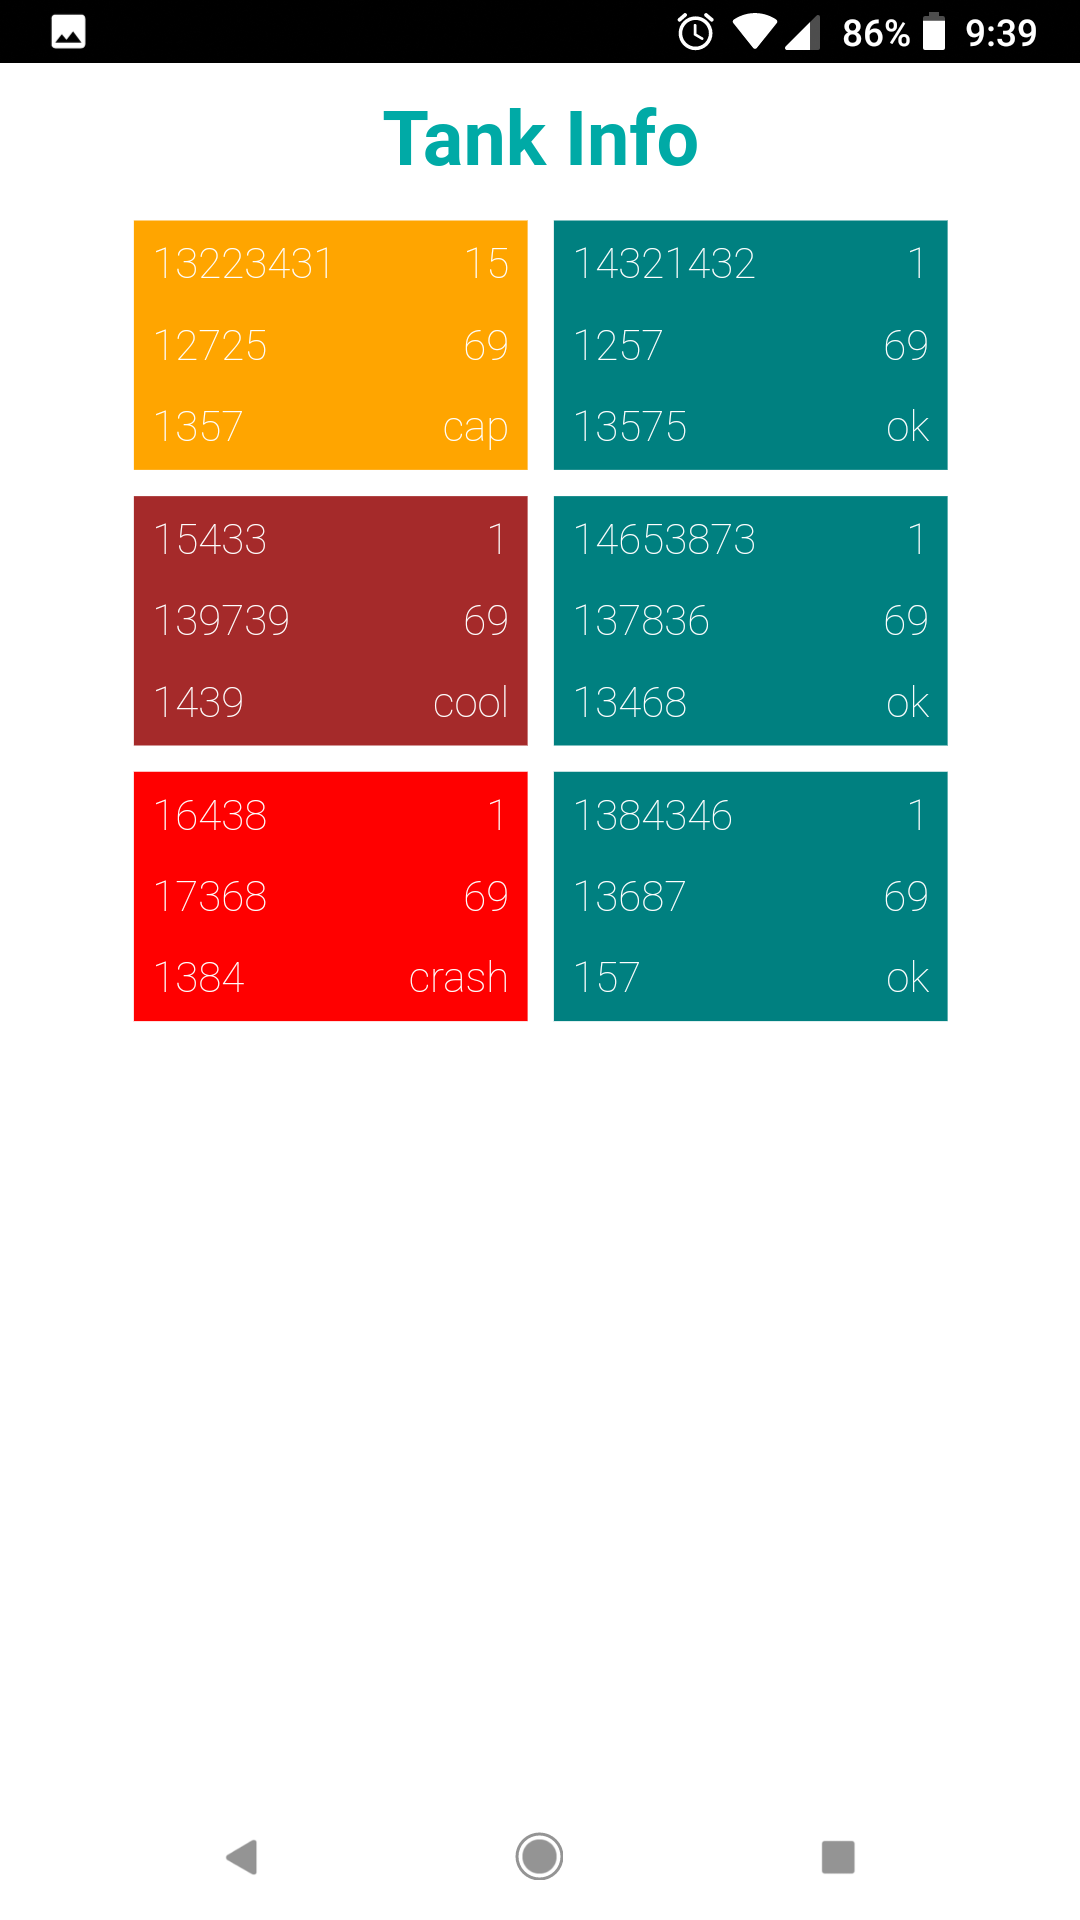
\includegraphics[height=13cm]{screenshots/mobile/tank_monitoring.png}}}%
    \qquad
    \subfloat[Tank Info]{{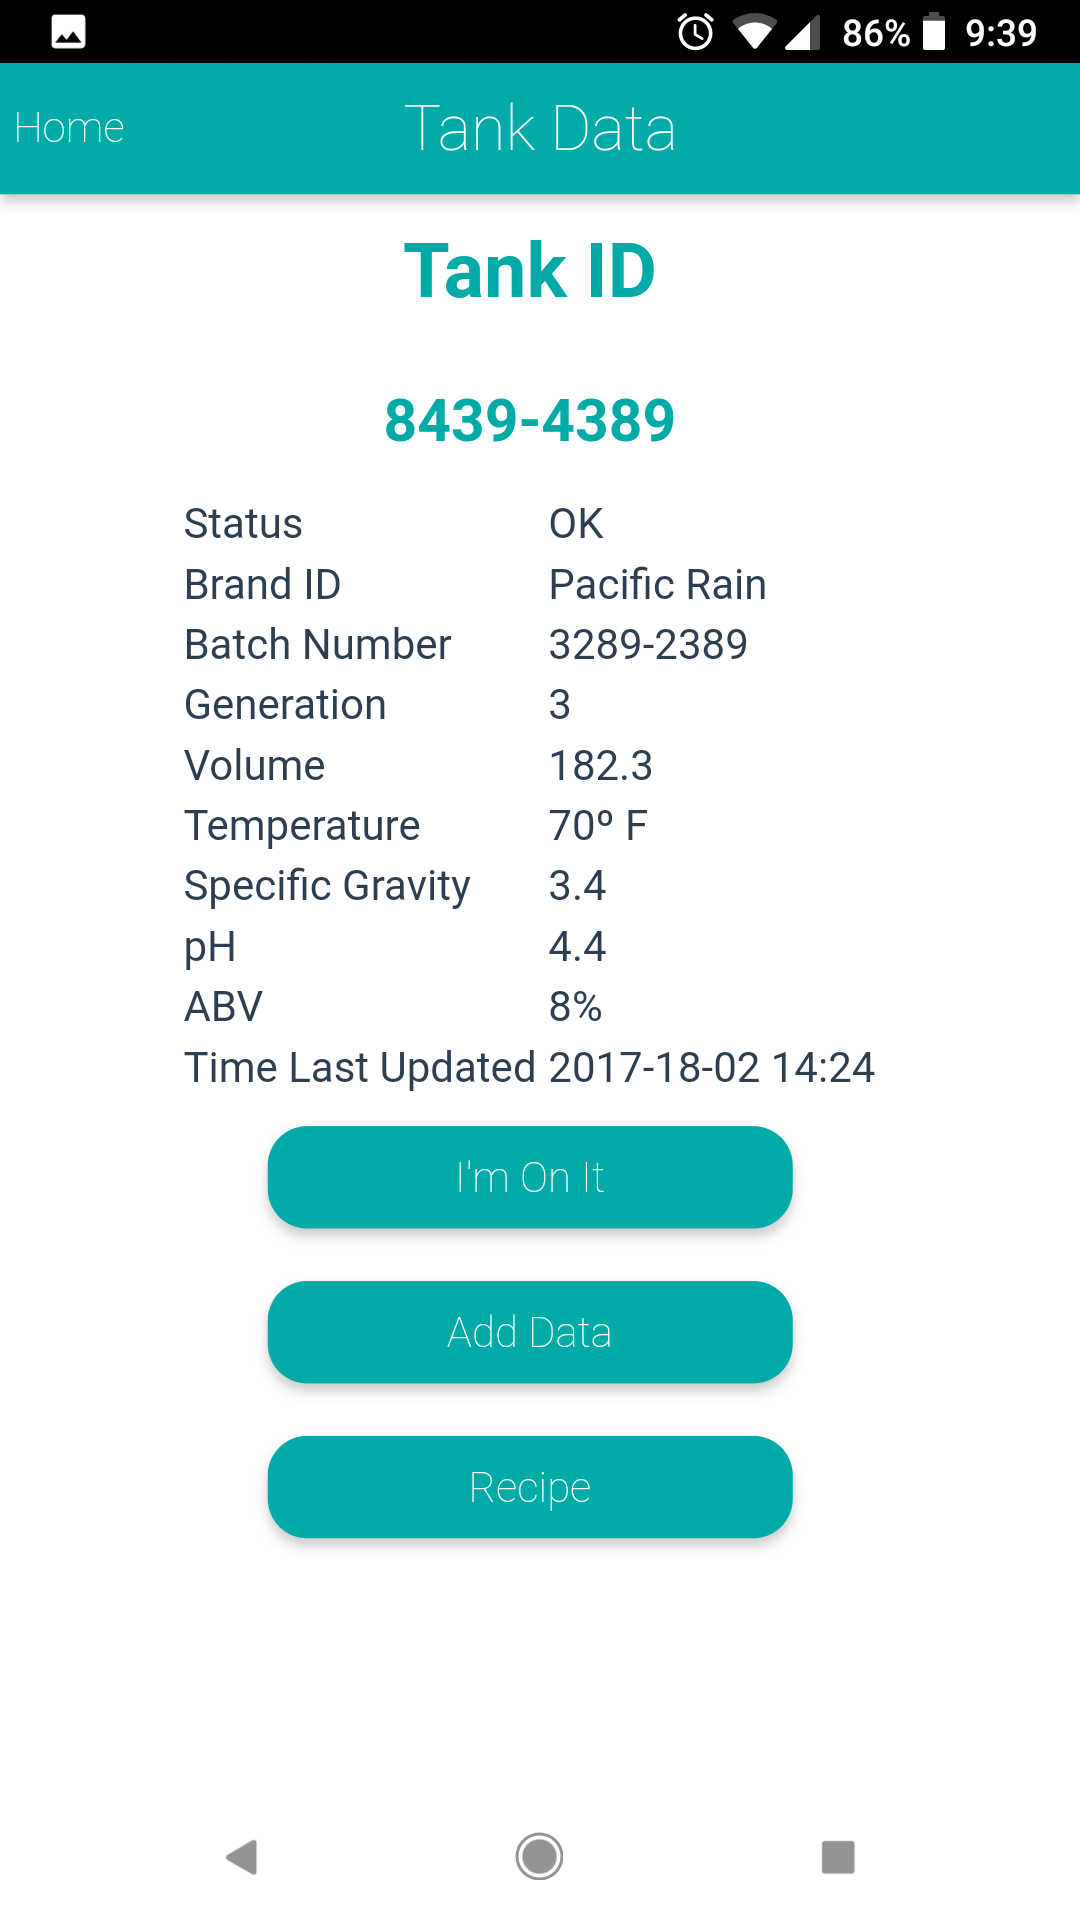
\includegraphics[height=13cm]{screenshots/mobile/tank_info.png}}}%
    \caption{Mobile - Tank monitoring and more info page}%
\end{figure}

\begin{figure}
	\centering
	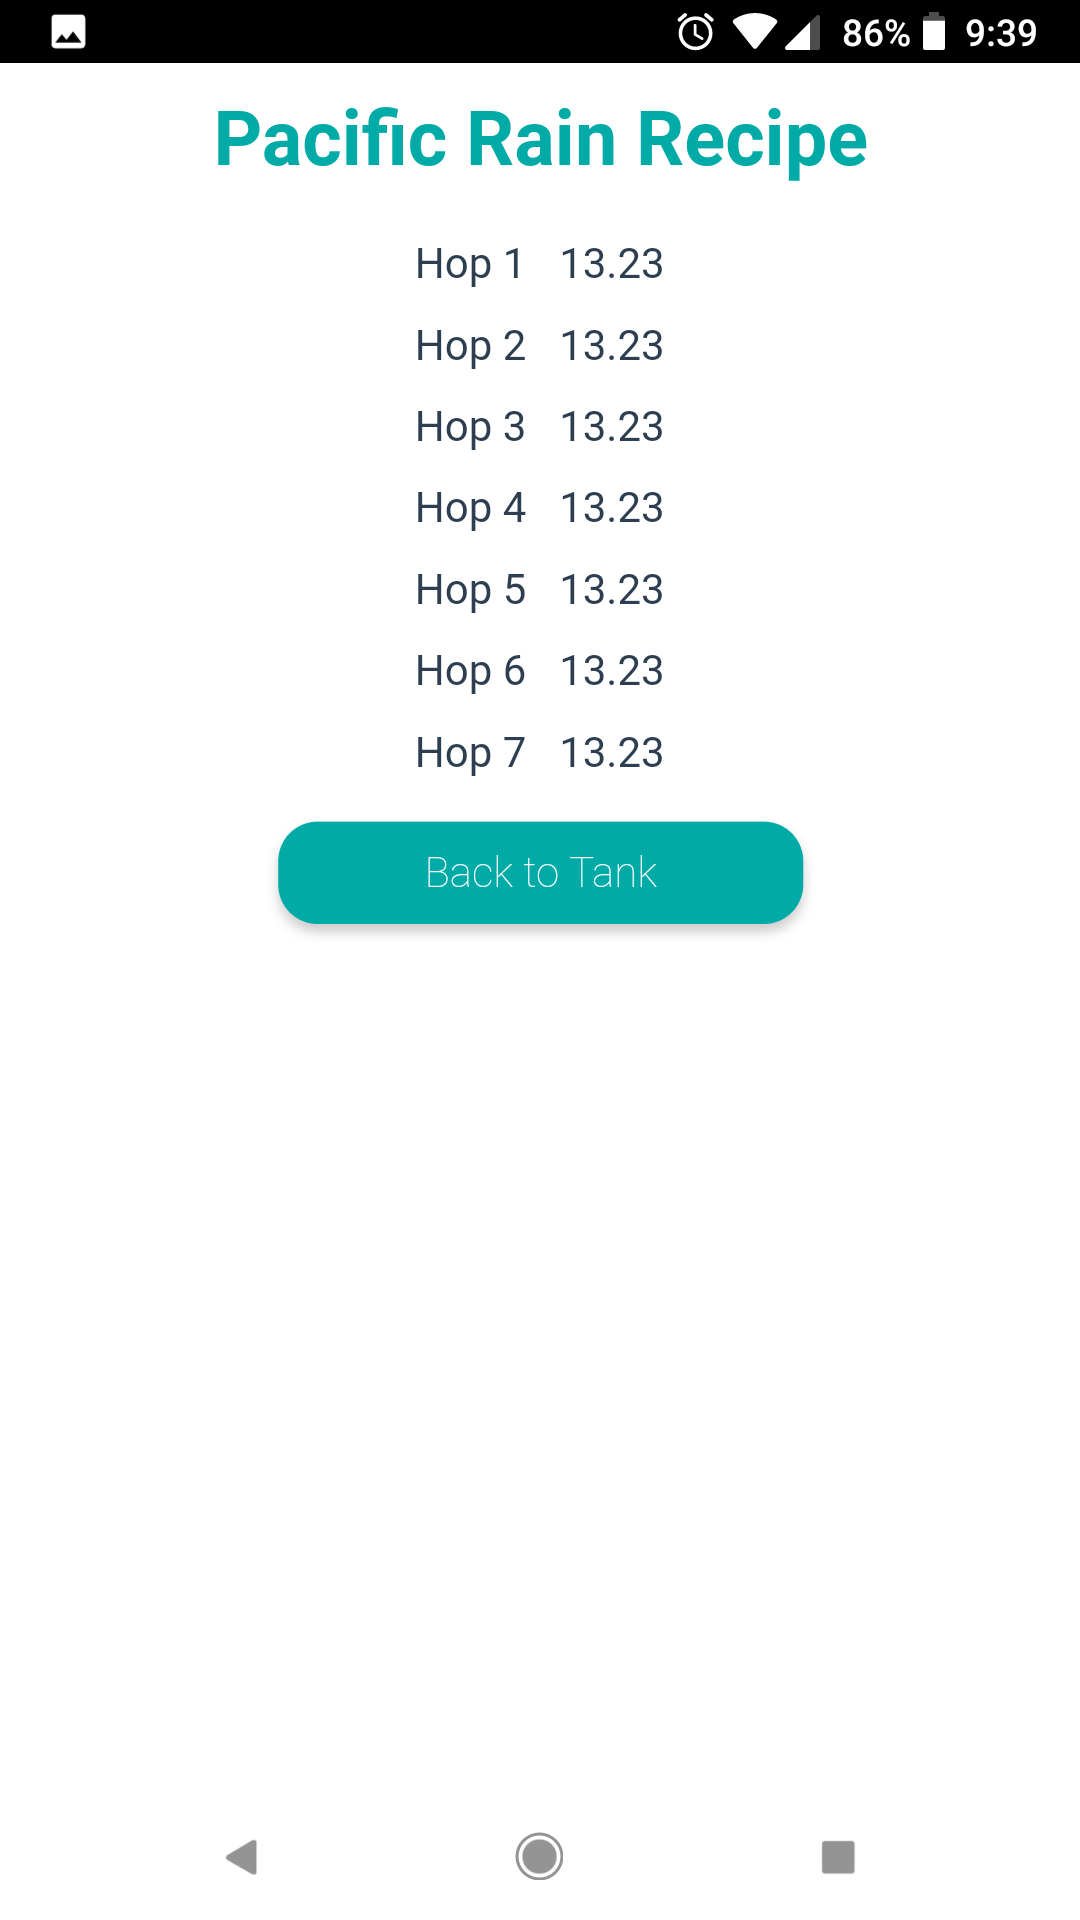
\includegraphics[height=13cm]{screenshots/mobile/recipe.png}
\end{figure}

\begin{figure}%
    \centering
    \subfloat[Data Entry]{{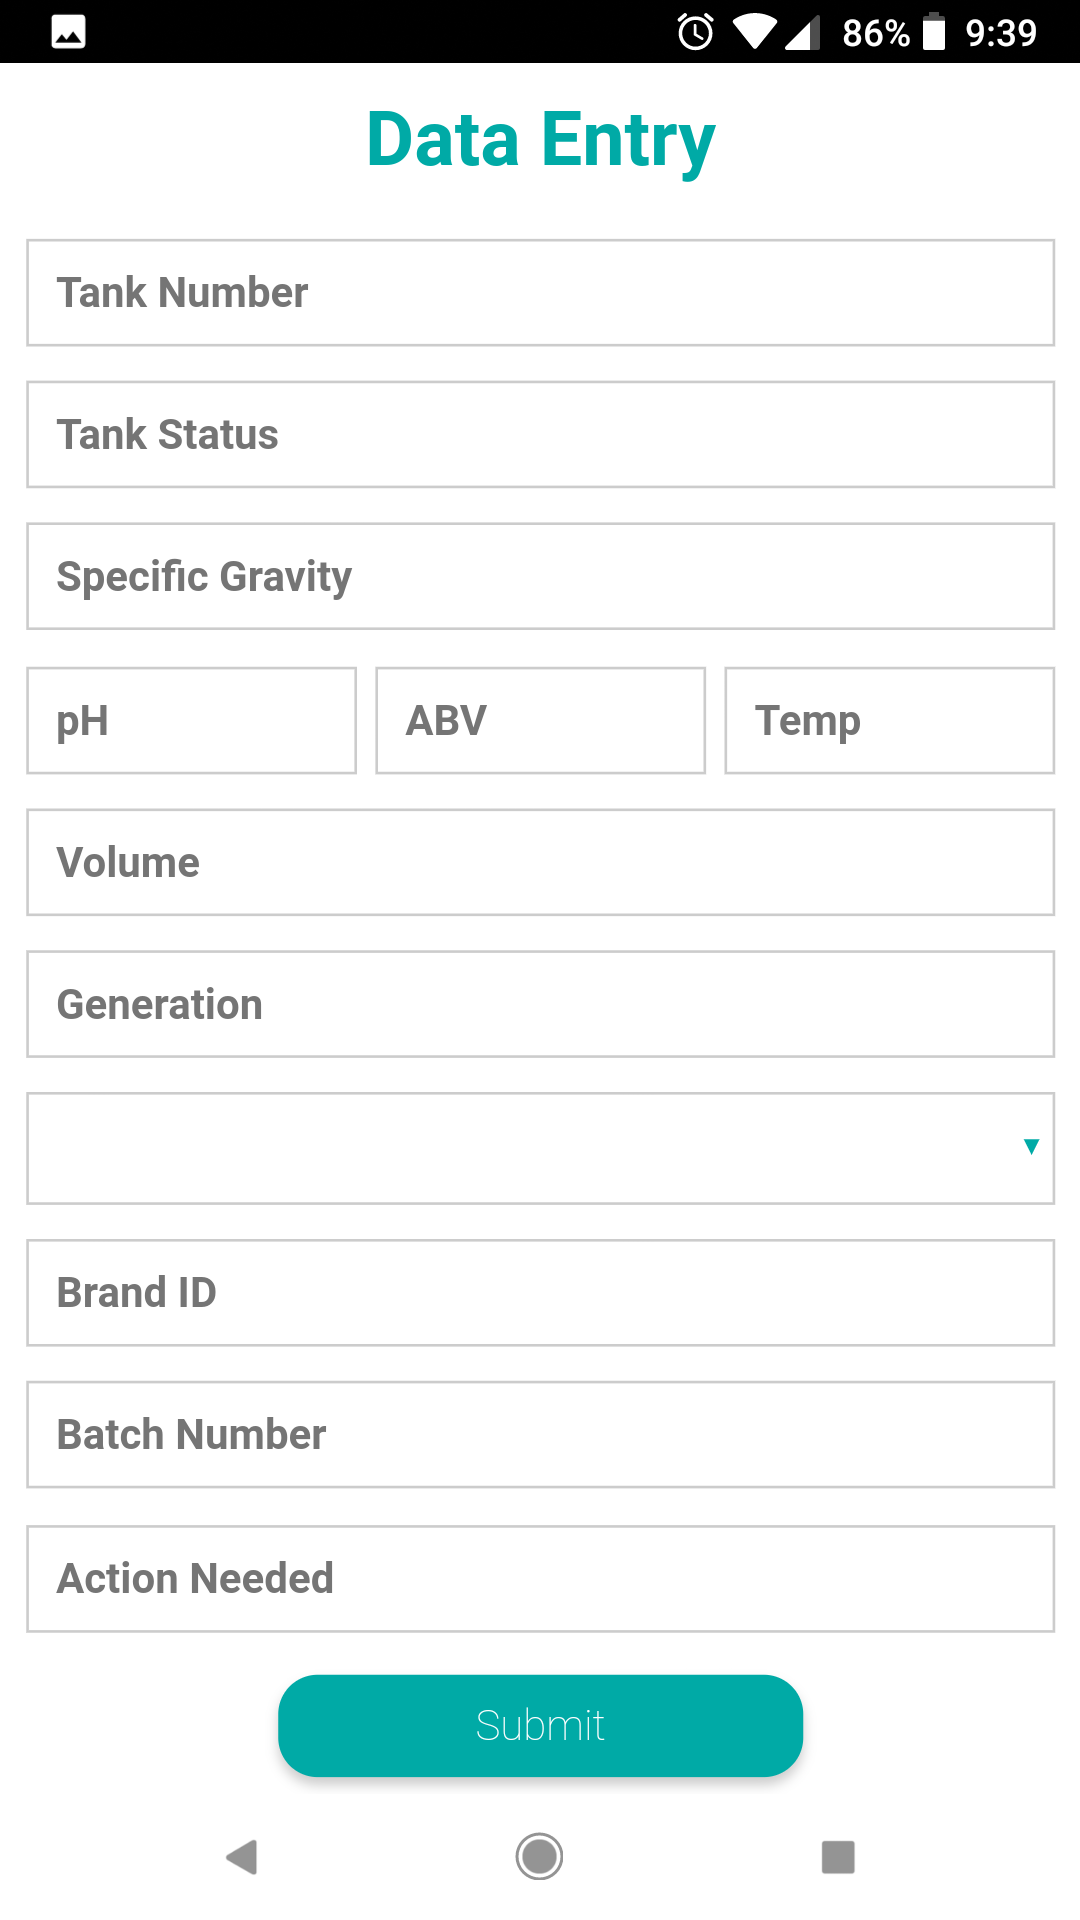
\includegraphics[height=13cm]{screenshots/mobile/data_entry.png}}}%
    \qquad
    \subfloat[Submission]{{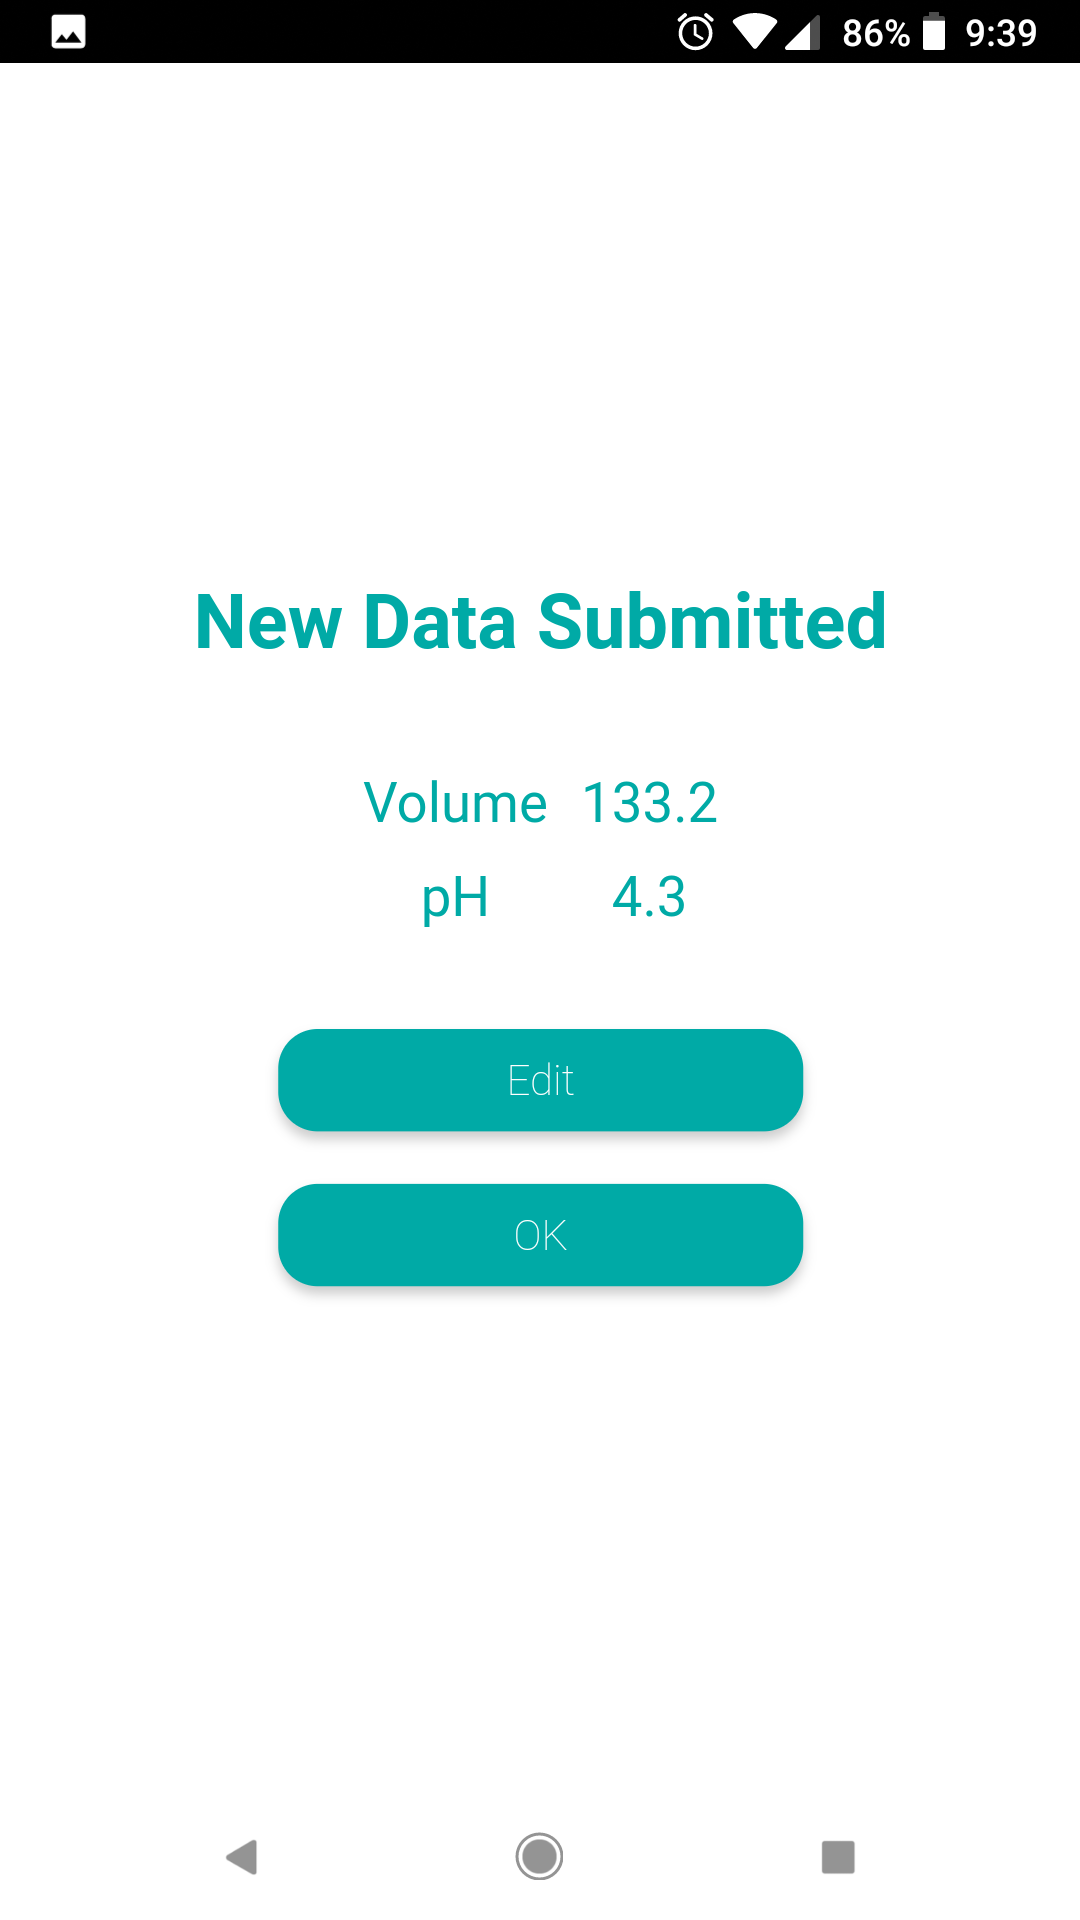
\includegraphics[height=13cm]{screenshots/mobile/submission.png}}}
    \caption{Mobile - Data entry and submission pages}%
\end{figure}

\end{document}
